\documentclass[a4paper,12pt]{article}
%

\usepackage{a4wide}
\usepackage{graphicx}
\usepackage{tikz}
\usetikzlibrary{shapes.geometric, arrows}
\usepackage[algo2e]{algorithm2e}
\usepackage{amsmath}
\usepackage{amsfonts}
\usepackage{amssymb}
\usepackage{multicol}
\usepackage{colortbl}
\usepackage{pgf,pgfarrows,pgfnodes,pgfautomata,pgfheaps,pgfshade}
\usepackage{gensymb}
\usepackage[utf8]{inputenc}
\usepackage[T1]{fontenc}
%\usepackage{dsfont}
\usetikzlibrary{shapes,trees}
\usetikzlibrary{graphs}
\usetikzlibrary{positioning}
\usetikzlibrary{arrows}
\usepackage{subcaption}
\usepackage[portuges]{babel}
\usepackage{siunitx}

\usepackage[utf8]{inputenc}
\usepackage[nottoc]{tocbibind}


%\usepackage[style=numeric]{biblatex}

%\addbibresource{relatorio.bib}

\begin{document}
%
\title{Trabalho final de AGE e OSD}


\author{R. Vieira\thanks{Departamento de Engenharia Mecânica, Universidade do Minho, {\tt ae5333@alunos.uminho.pt}}}

\maketitle              % typeset the header of the contribution

\begin{abstract}
O relatório apresenta o resultado da otimização de uma chapa em alumínio com dois objetivos e três parâmetros. Essa chapa é um elemento essencial de um sistema de teste para placas de circuito impresso sendo imperioso otimiza-la quanto ao peso e rigidez. Utilizou-se uma equação presente na literatura para modelar a deformação da chapa em funcionamento. Implementou-se um algoritmo genético NSGA-II utilizando uma livraria $open$ $source$ $Pymoo$. Este convergiu sem violação de restrições para uma frente de Pareto. Aplicando pesos concluiu-se que a solução ideal é encontrada para a deformação $0.0023m$ e massa $0.0023kg$ com os parametros $a=0.2500m$ $b=0.2500m$ e $h=0.0017m$.
\end{abstract}


\section{Introdução}

As placas de circuito impresso são essenciais numa era de crescente digitalização. É essencial garantir que não existem defeitos de produção para que operem normalmente na vida do componente. Para isso fazem-se testes com um sistema que mede tensões e correntes no circuito. Devido ao facto de os circuitos serem da ordem dos \SI{70}{\micro\metre} é essencial que este sistema de teste tenha uma alta rigidez (pouca deformação em operação) e de baixo peso (para que os operadores troquem o sistema de teste facilmente). 

O elemento mais importante desse sistema é uma chapa em Alumínio cujo comportamento mecânico pode ser modelado matematicamente. Assim, as funções objetivo (a minimizar) são:


\begin{equation}\label{eq:deform}
w_0= \sum_{n=1}^{\infty} \sum_{m=1}^{\infty} W_{mn} sin\left(\frac{m \pi x}{a}\right) sin\left(\frac{n \pi y}{b}\right)
\end{equation}

\begin{equation}\label{eq:mass}
Mass = a b h \rho_{material}
\end{equation}
\\
%\parencite[see][]{eqDeform}

Ou seja, a massa do sistema é modelado na equação~\ref{eq:mass} e os deslocamentos na equação~\ref{eq:deform}~\cite{eqDeform}. 
Sabendo que:

\begin{equation}\label{eq:fo}
D_{const}=\frac{E h^3}{12\left(1-{\nu}^2\right)}
\end{equation}

\begin{equation}\label{eq:fo}
k=\frac{k b^4}{D_{const} {\pi}^4}
\end{equation}

\begin{equation}\label{eq:fo}
\delta T=\frac{T \alpha D_{const} \left(1+\nu\right) {\pi}^2}{b^2}
\end{equation}

\begin{equation}\label{eq:fo}
W_{mn}=\frac{\frac{b^4}{D_{const} {\pi}^4} \left(q_{mn}+\delta T \left(m^2 s^2+n^2\right)\right)}{{\left(m^2 s^2+n^2\right)}^2+k}
\end{equation}

%\begin{equation}\label{eq:fo}
%\sigma_{max}=\frac{6q_mn\times2 b^2}{{\pi}^2 h^2 {\left(s^2+1\right)}^2} \left(s^2+\nu\right)
%\end{equation}

Para além disso, existem restrições técnicas sobre os três parâmetros geométricos. O comprimento e largura da chapa são limitados por limitação de espaço. O problema pode ser formalizado como:

\begin{equation}\label{eq:prob}
\begin{split}
\min\;\; &w_{0}(a, b, h)\\
\min\;\; &Mass(a, b, h)\\
s.a\;\; & 0.25\leq a\leq 0.5\\
& 0.25\leq b\leq 0.5\\
& 0.001\leq h\leq 0.01\\
\end{split}
\end{equation}

Onde $a$ e $b$ são os lados da chapa e $h$ é a sua espessura. Na figura~\ref{fig:defIm1}, vemos que a função deformação $w_{0}$ minimiza com a diminuição de $a$, $b$ e aumento de $h$. Nessa mesma figura é visivel que a função massa minimiza com os parâmetros $a$, $b$ e $h$. Ou seja, o parâmetro $h$ dá às funções um comportamento antagónico. Assim, o objetivo será conseguir um compromisso entre estas funções.

\begin{figure}[h]
\begin{center}
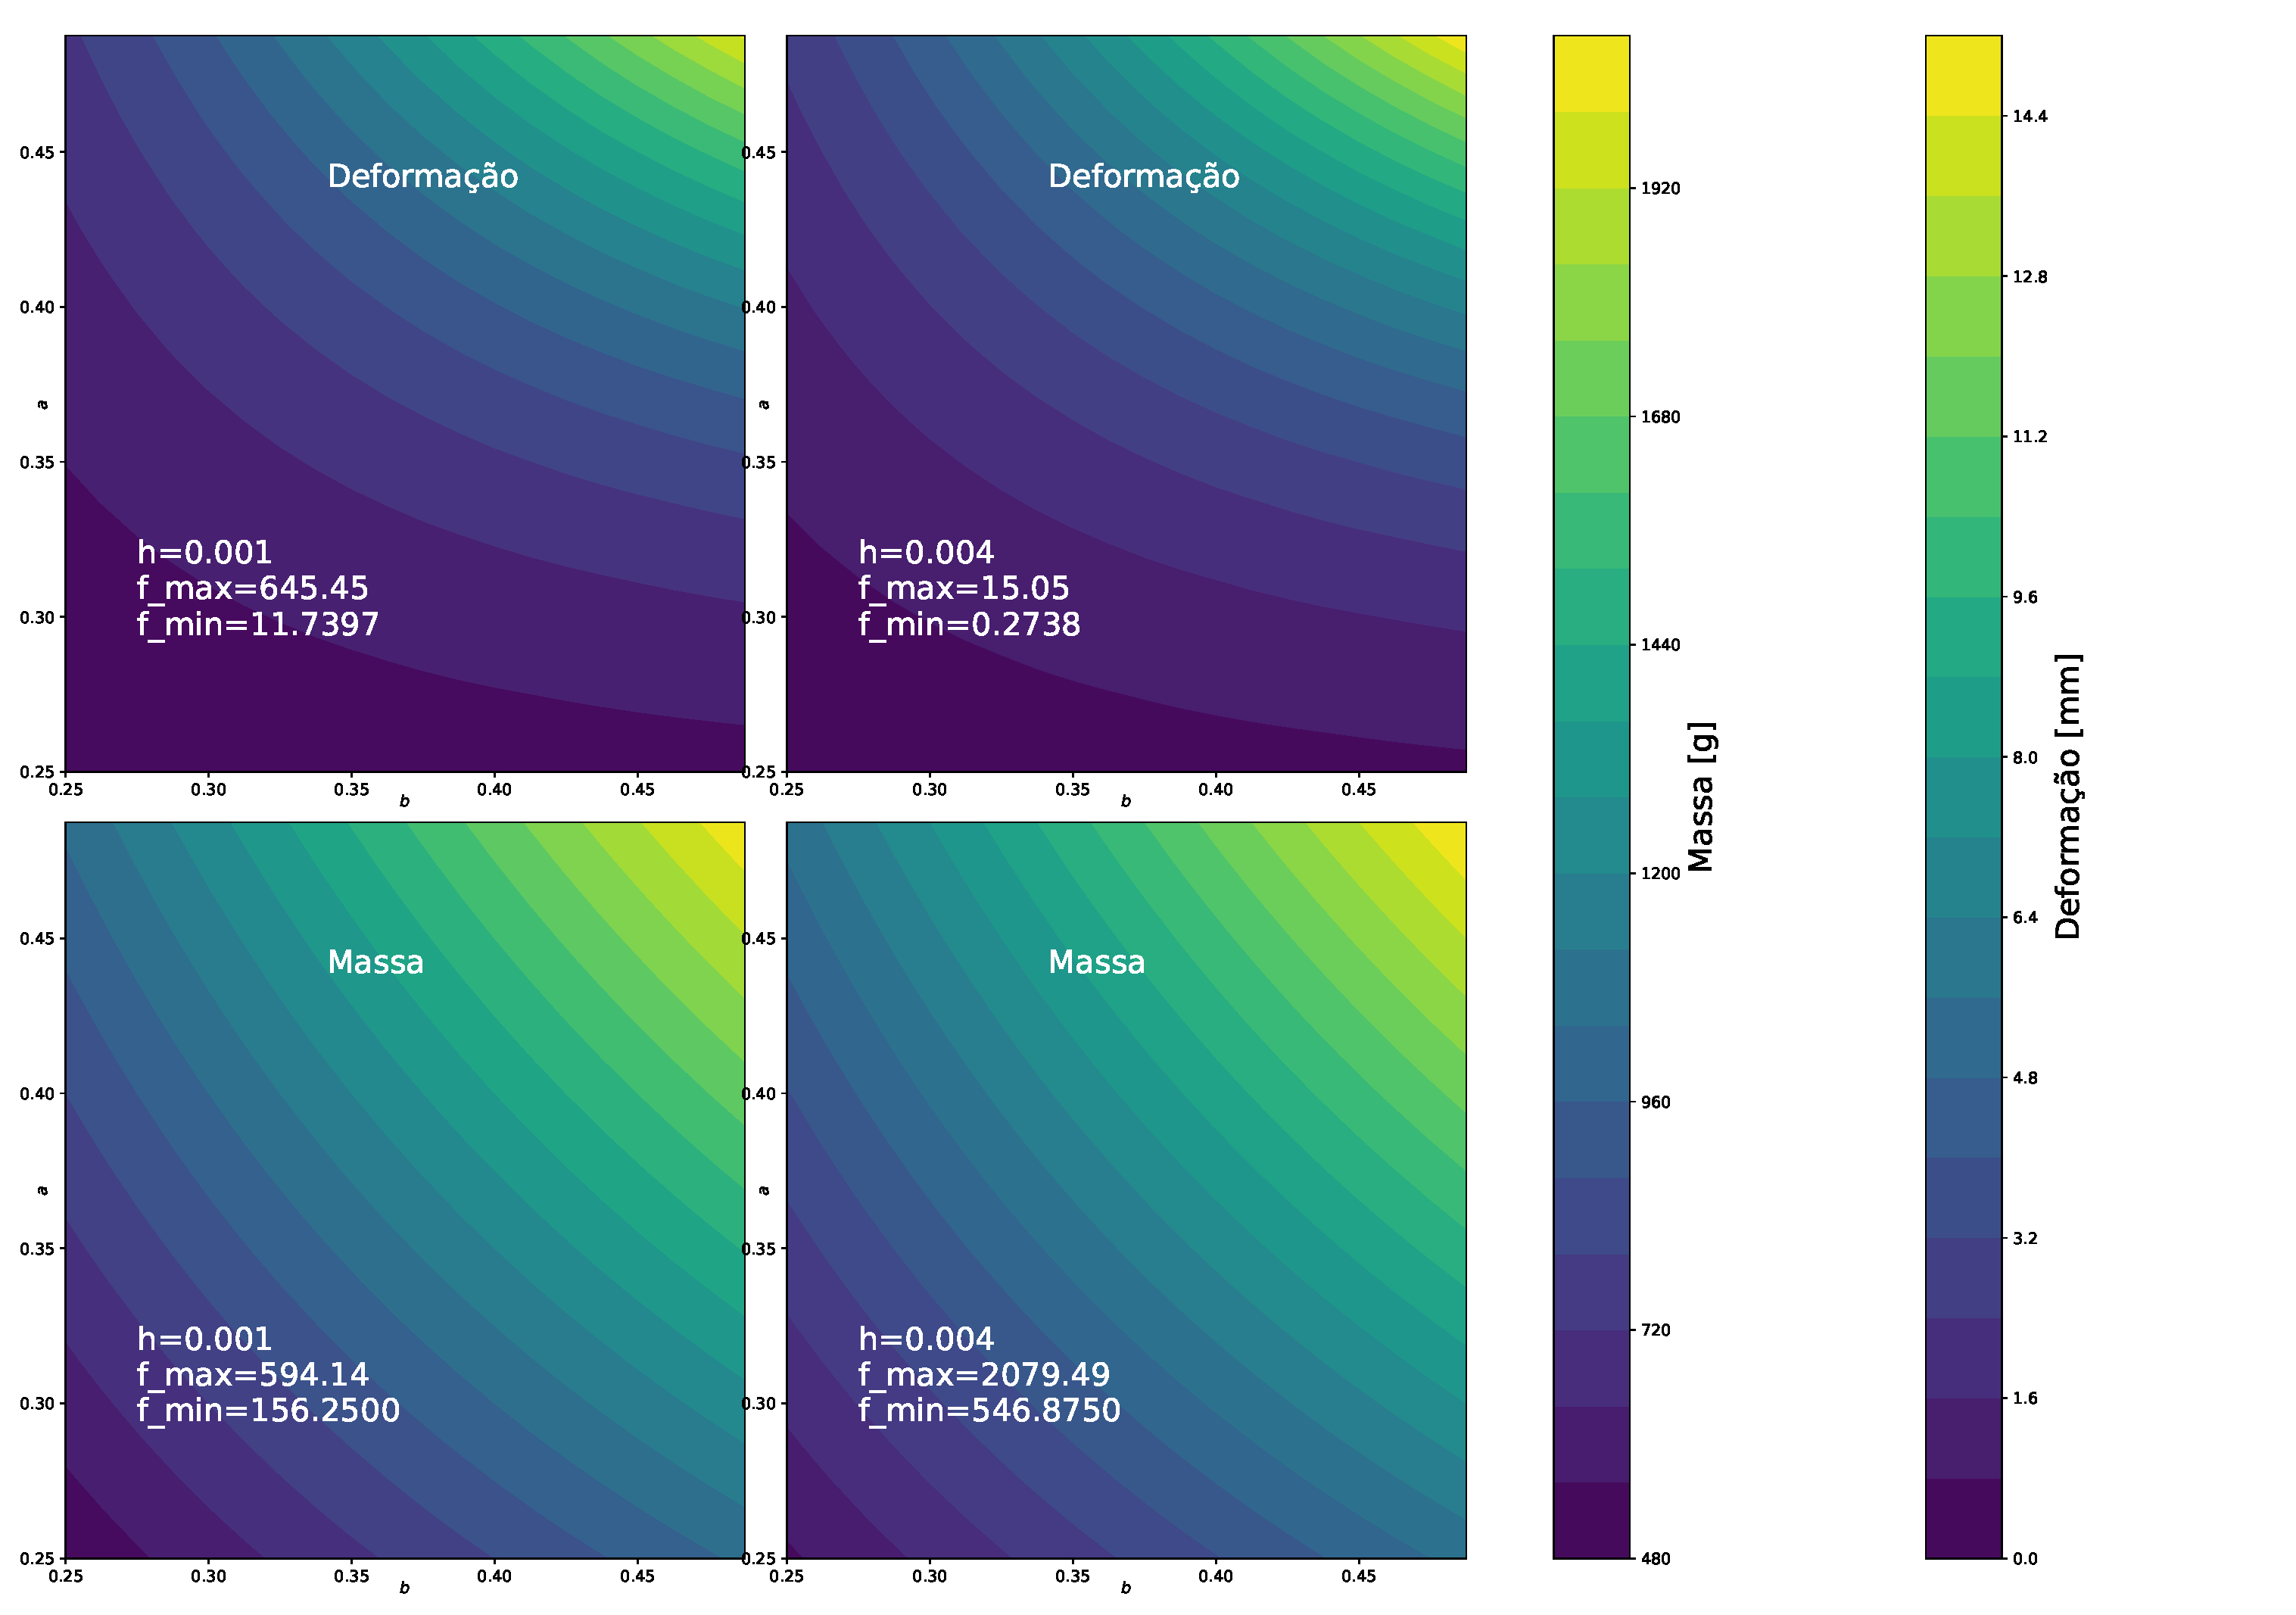
\includegraphics[scale=0.3]{deformacaoEmassa.eps}
\end{center}
\caption{A função massa e deformação desenhada com $h= 0.001, 0.004$}
\label{fig:defIm1}
\end{figure}

\section{Solução do problema com algoritmo genético}

A livraria utilizada foi o Pymoo~\cite{Pymoo} ~\cite{PymooArt} implementada para a linguagem de programação Python. Para resolver um problema multiobjetivo foi escolhido o algoritmo genetico NSGA-II~\cite{NSGA}. Este algoritmo utiliza uma estratégia elitista com partilha de parâmetros (isto é características) na população. Assim, uma população de n indivíduos gera uma população de descendentes através de uma selecção em torneio usando mutações para garantir variabilidade.

\subsection{Parametros do algoritmo relevantes}

Para o parâmetro $sampling$ for utilizado um campo aleatório. Foi definida uma população de 40 indivíduos com uma descendência de apenas 10. Esta é uma implementação ambiciosa que melhora a convergência em problemas relativamente simples. Para além disso foi ativada a opção que evita uma descendência igual à população original.

\subsection{Convergencia}

O metodo convergiu em 140 gerações. Visto que que neste problema temos apenas 3 parametros a variar podemos usar o $Hypervolume$ como um indicador de performance. Ele compara o ponto de referencia arbritario com a solução encontrada. Estabilidade deste indicador mostrado na figura~\ref{fig:hyper} ajuda a confirmar convergencia.


\begin{figure}[h]
\begin{center}
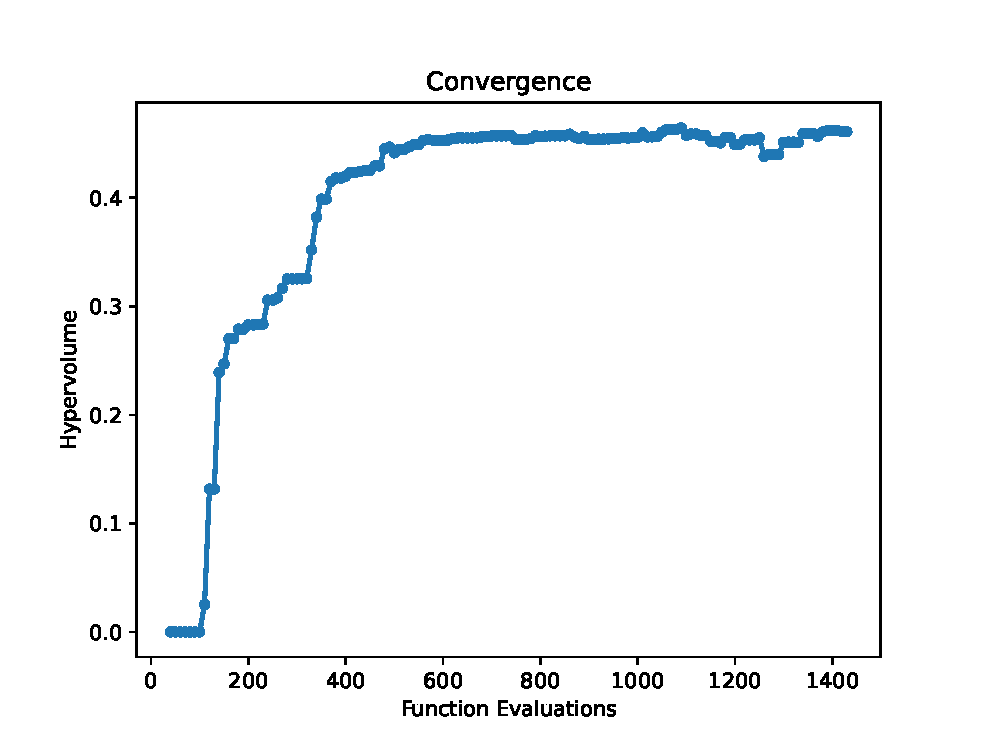
\includegraphics[scale=0.7]{convergence.eps}
\end{center}
\caption{Indicador $Hypervolume$ em função do numero de avaliações da função}
\label{fig:hyper}
\end{figure}

\subsection{Solução}

O resultado do método é um conjunto de soluções numa frente de Pareto, resta agora escolher aquela que é mais adequada. Para isso usou-se um método de decomposição, onde, utilizando uns pesos adequados em função da importância dos objetivos, o problema multidimensional é avaliado como se só existisse um objetivo. Na figura~\ref{fig:defIm2}, podemos ver esse $trade-off$ entre a massa do sistema e a sua deformação do sistema de teste.
Finalmente, solução ideal é encontrada para a deformação $0.0023m$ e massa $0.0023kg$ com os parametros $a=0.2500m$ $b=0.2500m$ e $h=0.0017m$.

\begin{figure}[!htbp]
\centering
\begin{subfigure}{.5\textwidth}
  \centering
  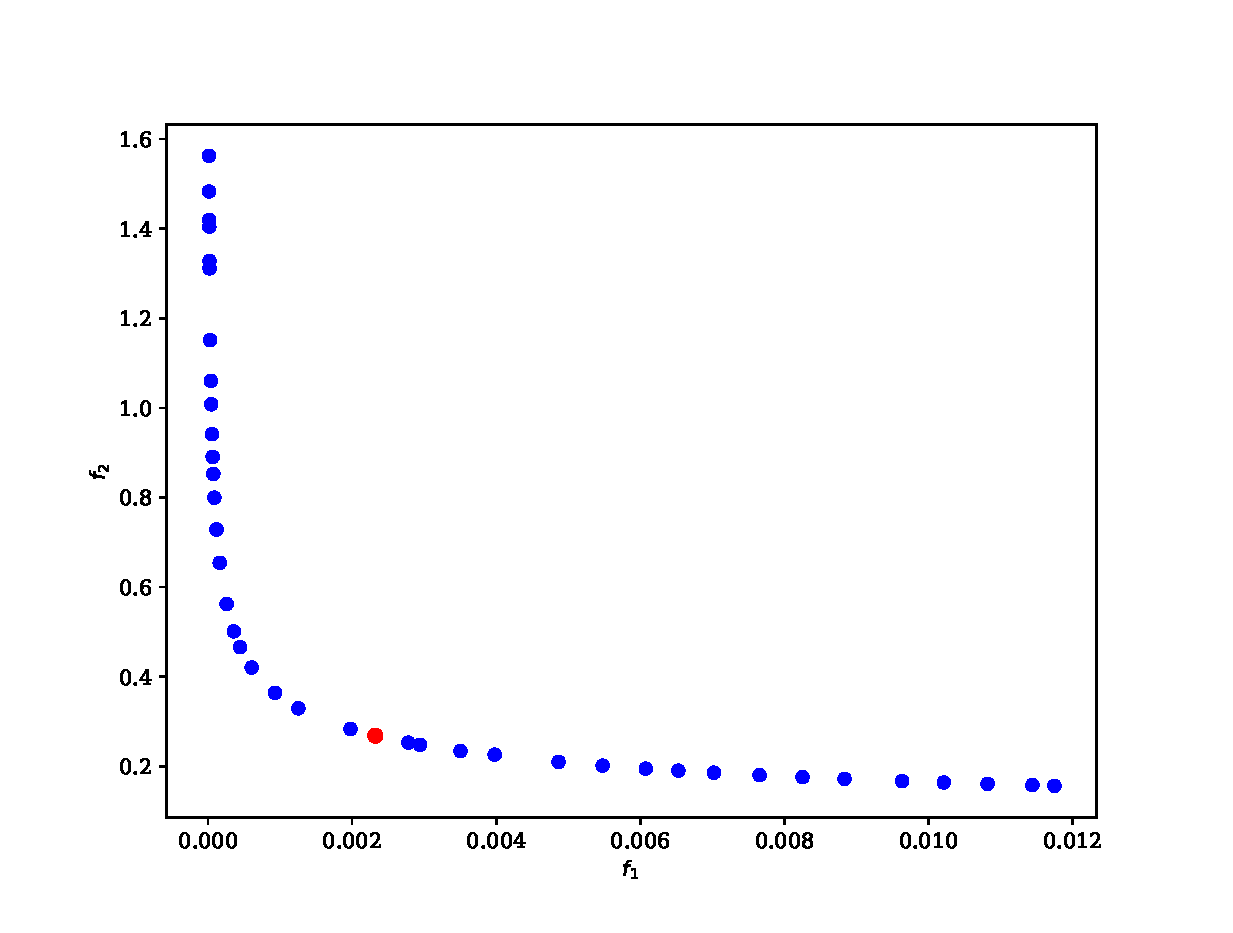
\includegraphics[width=.99\linewidth]{objSpace.eps}
  \caption{Frente de Pareto}
  \label{fig:sub1}
\end{subfigure}%
\begin{subfigure}{.5\textwidth}
  \centering
  
\includegraphics[width=.99\linewidth]{parallel_coord.eps}
  \caption{Soluções em coordenadas paralelas}
  \label{fig:sub2}
\end{subfigure}
\caption{\label{fig:defIm2}A solução mais equilibada está a vermelho}
%\label{fig:test}
\end{figure}


\section{Solução do problema com procura coordenada}

Algoritmos de procura coordenada são métodos numéricos de optimização que não requerem gradientes. Essencialmente, o algoritmo varia um parametro teórico com passos com a mesma magnitude, é determinada a direcção que minimiza a função, o passo é divido por 2 e o processo é repetido até que os passos são considerados suficientemente pequenos. Para o problema foi escolhido algoritmo de Hooke and Jeeves.


\subsection{Parametros do algoritmo relevantes}

Os parametros mais relevantes são os coeficientes exploratórios e o comprimento 

%	explr_delta=0.1, 
%	explr_rho=0.1, 
%	pattern_step=2, 
%	eps=1e-12, 


\subsection{Solução}

O resultado do método é um conjunto de soluções numa frente de Pareto, resta agora escolher aquela que é mais adequada. Para isso usou-se um método de decomposição, onde, utilizando uns pesos adequados em função da importância dos objetivos, o problema multidimensional é avaliado como se só existisse um objetivo. Na figura~\ref{fig:defIm2}, podemos ver esse $trade-off$ entre a massa do sistema e a sua deformação do sistema de teste. A solução ideal é encontrada para a deformação $0.0043m$ e massa $0.0043kg$ com os parametros $a = 0.2840$ $b = 0.3016$ e $h = 0.0020$.



\begin{figure}[!htbp]
\centering
\begin{subfigure}{.5\textwidth}
  \centering
  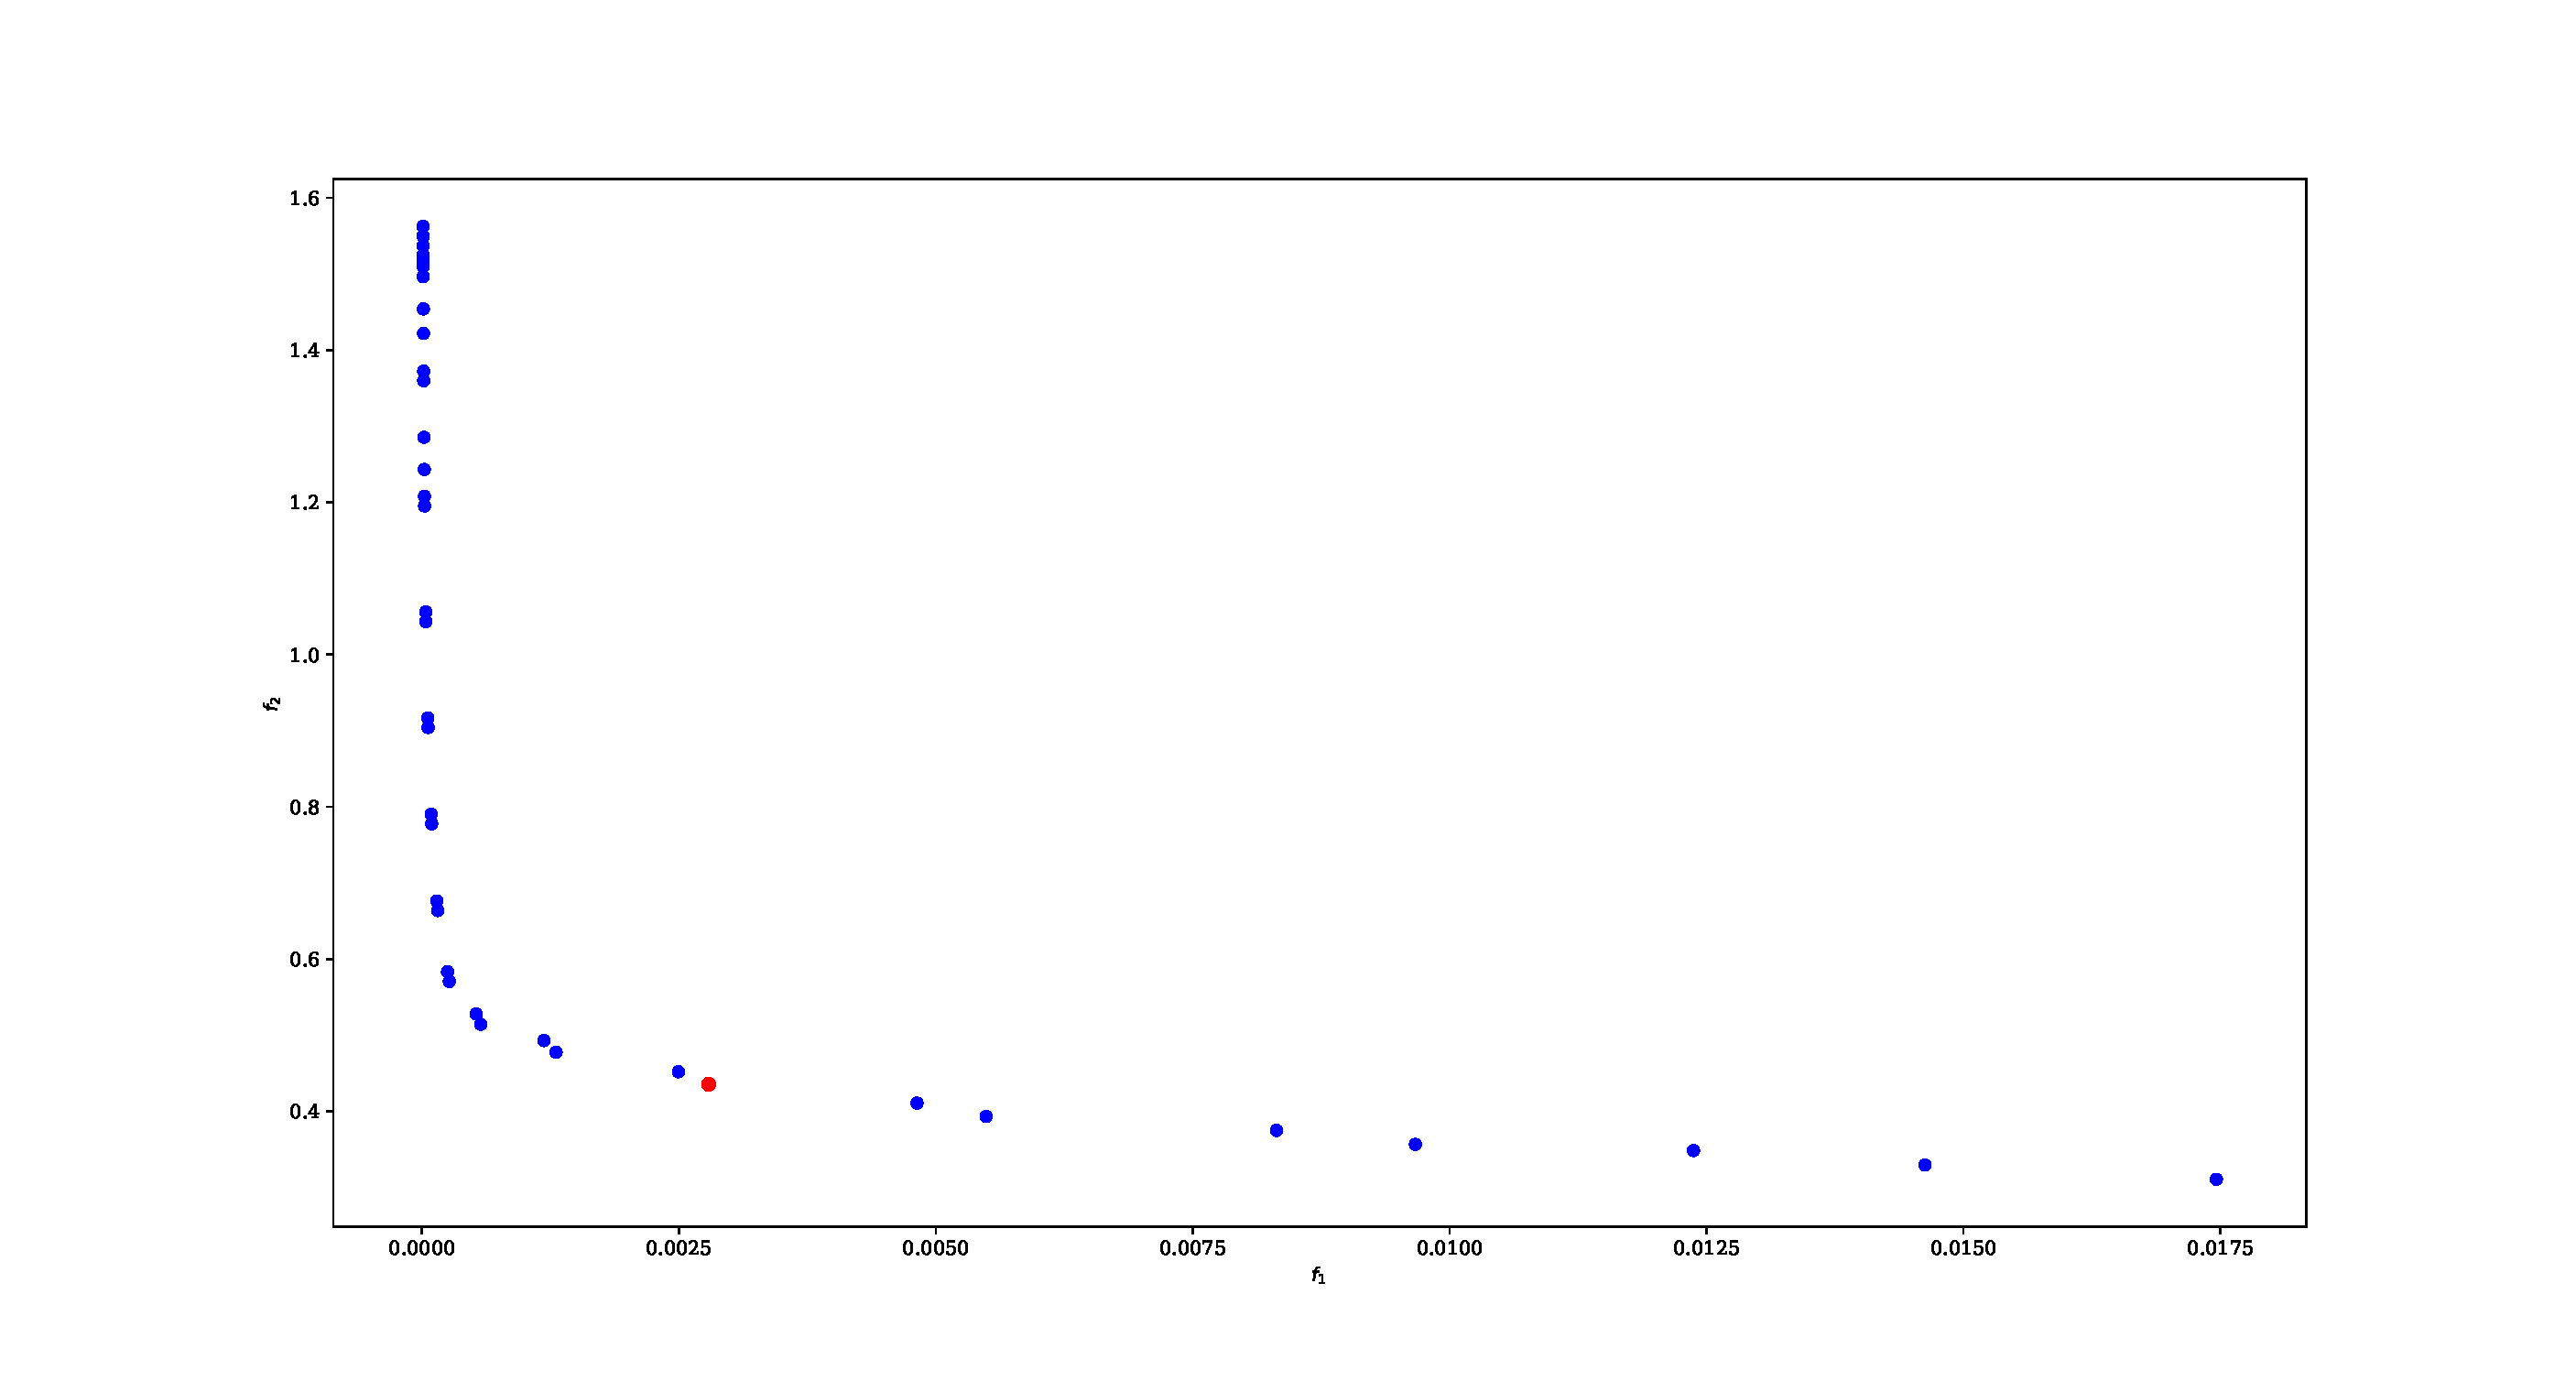
\includegraphics[width=.99\linewidth]{PS_objSpace.eps}
  \caption{Frente de Pareto}
  \label{fig:sub1}
\end{subfigure}%
\begin{subfigure}{.5\textwidth}
  \centering
  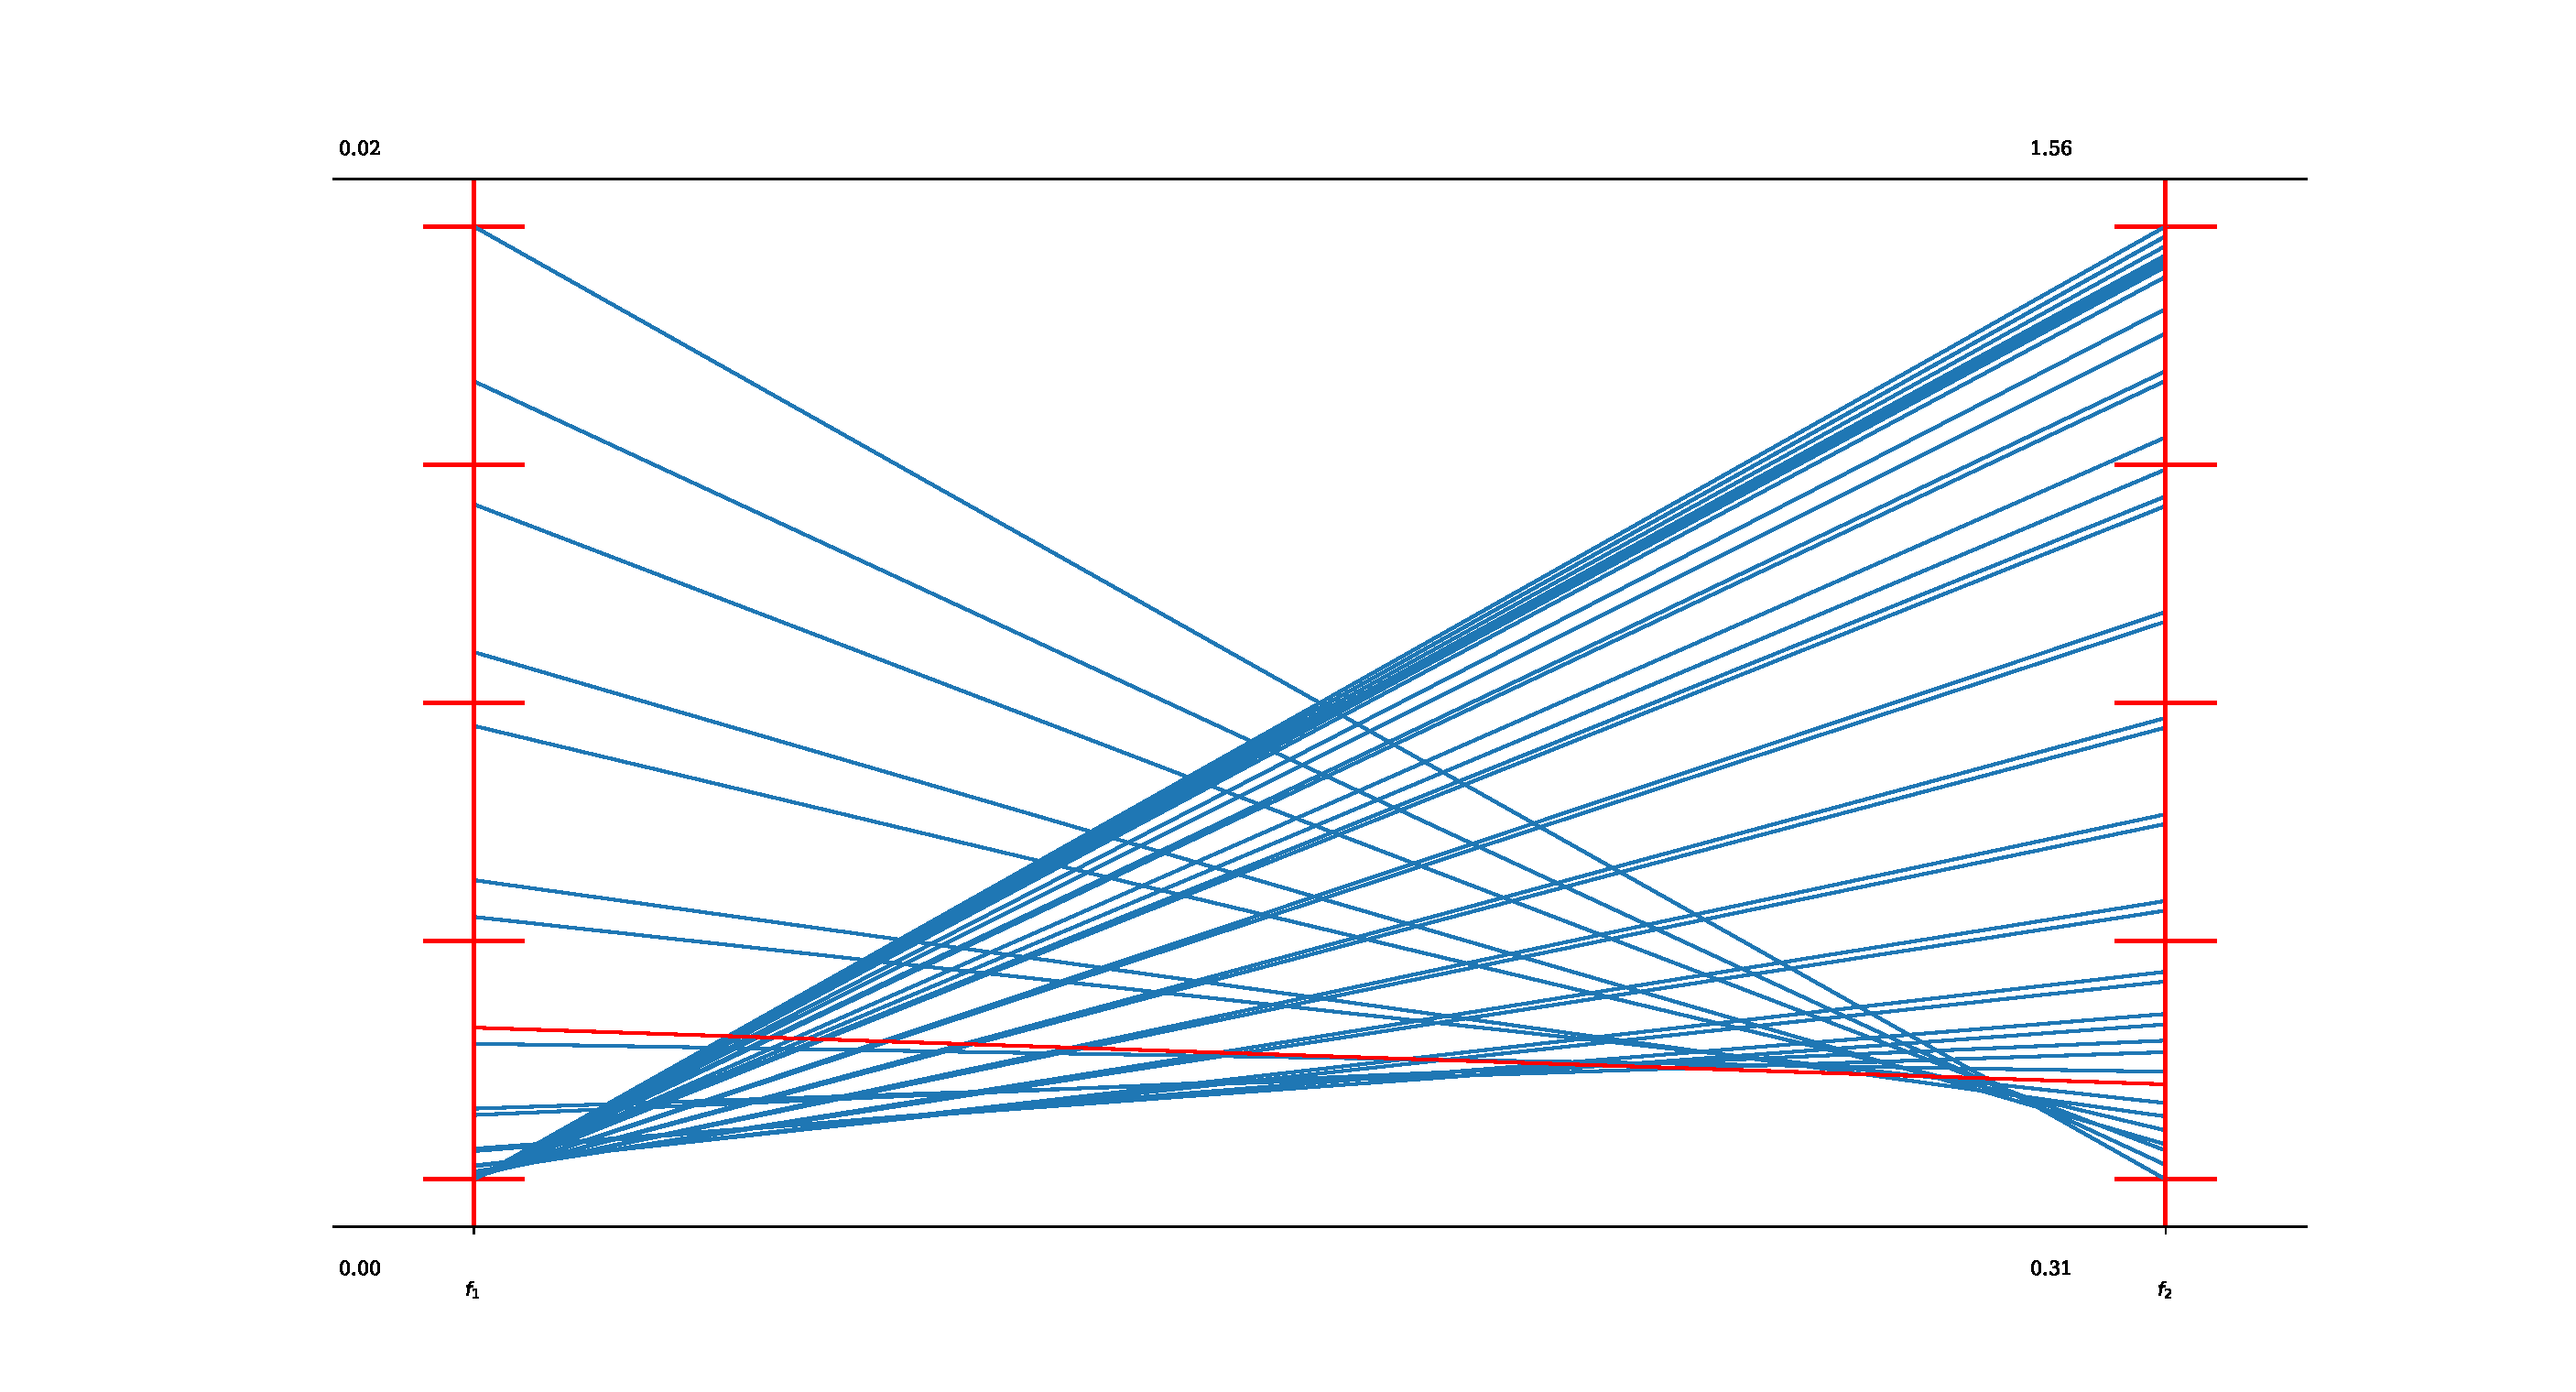
\includegraphics[width=.99\linewidth]{PS_parallel_coord.eps}
  \caption{Soluções em coordenadas paralelas}
  \label{fig:sub2}
\end{subfigure}
\caption{\label{fig:defIm2}A solução mais equilibada está a vermelho}
%\label{fig:test}
\end{figure}



\section{Conclusões}

A livraria Pymoo é uma interessante ferramenta $open source$ que implementa em C os principais algoritmos de otimização, com um API em python que torna a sua utilização simples flexível e com uma boa performance computacional.\\
A escolha do algoritmo NSGA-II foi o correto para este tipo de problema, com uma convergência suave sem violações de restrições durante o processo de calculo.\\
Com a análise da figura~\ref{fig:defIm2} é possível verificar que a aplicação de pesos num método de decomposição permitiu obter uma solução equilibrada, evitando soluções na frente de Pareto que privilegiem apenas um dos objetivos.\\

\newpage

\appendix

\section{O código}\label{A:1}

Neste apêndice está uma parte do código fonte que pode ser consultado na sua totalidade em:\\ https://github.com/RuiVieira89/top4ICT\\
\\
Aqui podemos ver a implemtação do modelo com os seus principais parâmetros.

\begin{verbatim}
from pymoo.model.problem import Problem

class MyProblem(Problem):

	def __init__(self):
		super().__init__(n_var=3, 
			n_obj=2,
			n_constr=2,
			xl=np.array([0.25, 0.25, 0.001]),
			xu=np.array([0.5, 0.5, 0.01]),
			# elementwise_evaluation=True
			)

	def _evaluate(self, X, out, *args, **kwargs):

		w, sigma_max = function(X) 
		sysMass = np.prod(X, axis=1)*MaterialDensity

		out["F"] = np.column_stack([w, sysMass])
		out["G"] = np.column_stack([-w,-sysMass])


problem = MyProblem()

from pymoo.algorithms.nsga2 import NSGA2
from pymoo.factory import get_sampling, get_crossover, get_mutation
from pymoo.algorithms.so_genetic_algorithm import GA

algorithm = NSGA2(
	pop_size=40,
	n_offsprings=10,
	sampling=get_sampling("real_random"),
	crossover=get_crossover("real_sbx", prob=0.9, eta=15),
	mutation=get_mutation("real_pm", eta=20),
	eliminate_duplicates=True
)

from pymoo.util.termination.default import MultiObjectiveDefaultTermination

termination = MultiObjectiveDefaultTermination(
    x_tol=1e-8,
    cv_tol=1e-6,
    f_tol=0.0025,
    nth_gen=5,
    n_last=30,
    n_max_gen=1000,
    n_max_evals=100000
)

from pymoo.optimize import minimize

res = minimize(problem, 
	algorithm, 
	termination, 
	seed=1, 
	save_history=True, 
	verbose=True
	)
\end{verbatim}



\bibliographystyle{plain.bst}
\bibliography{relatorio}


\end{document}